\chapter{Phase Retrieval}
The problem of missing phase information is well known and is called the phase problem. There are many ways to overcome it: for example in crystallography homology modelling or the anomalous scattering of heavy atoms is exploited to retrieve phases. Holography uses the interference between two wave fields to obtain the phases. Ptychography uses the precisely known overlap and high redundancy between many exposures to solve the phase problem. In CXI the scattered field gets oversampled, which means that phases can under certain conditions be retrieved from the intensity pattern itself. The next sections will describe oversampling in more detail, explain how phases can be retrieved from an oversampled signal using an iterative phase retrieval method, and finally how phase retrieval can be validated. 

\section{Oversampling} 
In 1952 Sayre noticed that the Bragg peaks sample the molecular transform $\mathcal{F}(H)$ at the critical sampling rate ($S_C$)\cite{Sayre1952a} (See Shannon \cite{Shannon1949a}). This means that knowing the phases belonging to the Bragg peaks is just enough to back-calculate the structure of the measured object. Single particle imaging is free from the crystal lattice, and isolated Bragg peaks give way to a continuous diffraction pattern. By choosing the detector distance appropriately such that individual pixels cover a small enough angle, we can sample the molecular transform more finely than the critical sampling rate. This sampling condition is called oversampling. Figure \ref{fig:sampling} illustrates both cases of sampling. 

\begin{figure}[h]
	\centering 
		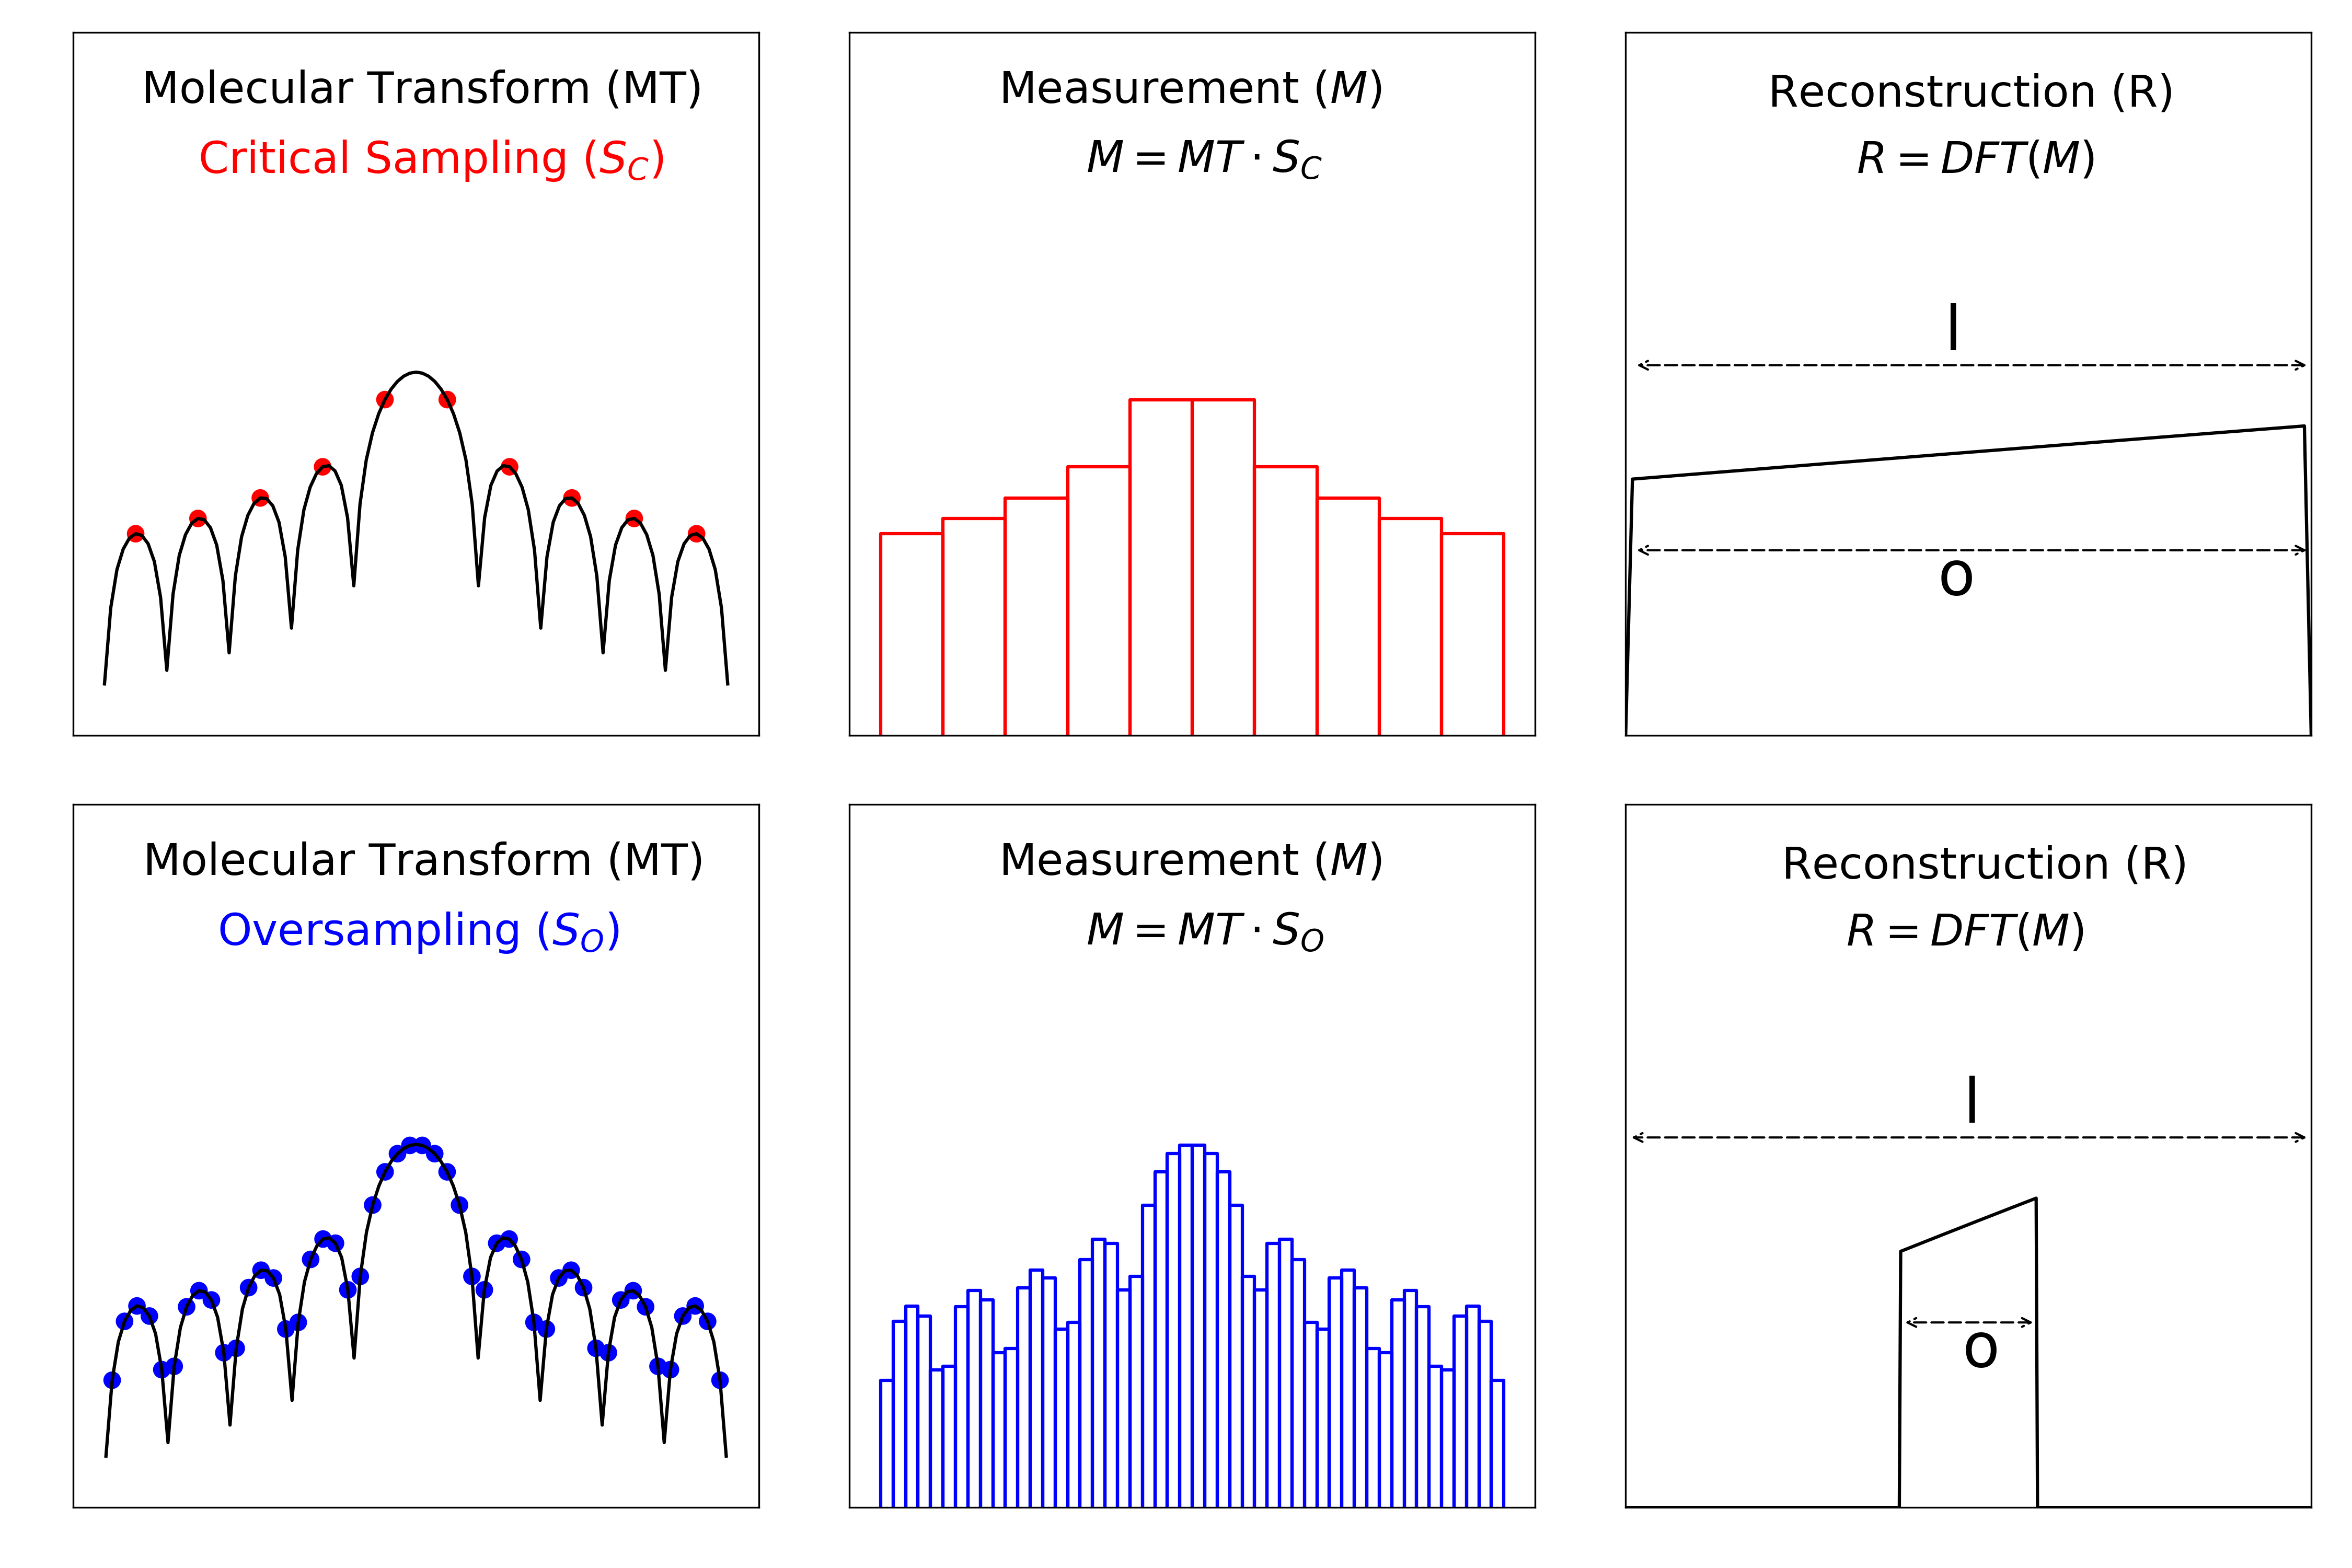
\includegraphics[width=120mm]{sampling.png}
	\caption{Illustration of critical sampling versus 		oversampling.}
	\label{fig:sampling}
\end{figure}

The linear sampling rate $S$ is defined as the ratio of $l/o$, where $l$ is the window size, and $o$ is the object size. Due to the inverse relation between the object and the molecular transform $l = \frac{1}{q} = \frac{\lambda\, d}{p}$, where $q$ is a pixel in the molecular transform (see equation \ref{eq:q}). 

\begin{equation}
S = \frac{\lambda\,d}{o\,p}
\end{equation}

By choosing a detector setup such that the sampling rate is at least twice the critical sampling rate we can, in some cases, use the additional intensity information to recover the phases, and thus reconstruct the object from the measured intensities alone. It is known that this method does often does have multiple solutions in 1D \cite{Walther1963}, however, for higher dimensions it has been proven that, in most cases, an oversampled pattern will have a unique solution\cite{Bruck1979}. Oversampling is the basis of many phase retrieval techniques in SPI, as well as some clever phasing techniques in SFX \cite{Ayyer2016,Chapman2011}.

\section{Iterative Phase retrieval}
In practice there are many ways of possibly retrieving the phase information from the diffraction pattern, but most common phase retrieval techniques are variations of convex optimization algorithms. This section introduces the general idea behind convex optimization, and explains the working three different algorithms. It has to be appreciated that solving the phases problem in remarkably difficult. It is neither linear nor convex.

As with any difficult problem, one starts from the things that are known. Figure \ref{fig:sampling} shows that oversampling in Fourier space implies that there is an area the size of ($l-o$) around the object for which we know the electron density $\rho(\vec{r})$ is zero. This knowledge can be used as a constraint on the possible phases: we know that a correct choice of phases would make the corresponding $\rho(r)$ be zero in this area. The area that can contain positive electron density is called the support mask $M(\vec{r})$. This constraint is called the real-space constraint. Furthermore, we know that the recovered Fourier amplitudes should agree with the measured intensities. This is called the Fourier-space constraint. 

In 1978 Fienup \cite{Fienup1978}, inspired by an earlier algorithm by Gerchberg and Saxton [Gerchberg1972], introduced an algorithm called Error Reduction (ER) to solve the phase problem. ER is an iterative approach that tries to find the solution that minimizes the disagreement to both the real-space constraint and the Fourier constraint. In words it can be described as follows:\\
\begin{enumerate}
\item Assign random phases to each pixel.
\item Inverse Fourier transform F(s).
\item Set all electron density outside of $M$ to zero, keep other electron density.
\item Fourier transform $\rho(r)$
\item Make sure that the recovered amplitudes match the measured intensities. Keep the phases.
\item Go back to step 2.\\
\end{enumerate}


ER is sometimes able to find the correct solution, but because the problem is not convex, in general it often gets stuck in local minima, making ER unable to find the global solution.

In 1984 Levi and Stark realized that applying the above described constraints can be interpreted as projections in a multidimensional Hilbert space \cite{Stark1984}. Step 3 will from now on will be called the real-space projection $P_r$. A combination of step 4,5 and 2 will be called the Fourier Projection $P_f$.  In ER $P_r$ and $P_f$ can be defined as follows:
\begin{align}\label{eq:ER}
P_r \rho\left(\vec{r}\right) =& \begin{cases} \rho\left(\vec{r}\right) \quad &\mathrm{if}\,\,
    \vec{r} \in M\\0 \quad & \mathrm{if}\,\, \vec{r} \not\in M \end{cases}\\
P_f \rho(\vec{r}) =& \mathcal{F}^{-1}\left( \frac{\sqrt{I}}{|\mathcal{F}(\rho(\vec{r}))|}\mathcal{F}(\rho(\vec{r})) \right)
\end{align}

The largest difference between both projections is that the support constraint is convex, while the Fourier constraint is not. An iteration in ER can now been seen as a real-space projection followed by a Fourier projection. This can be summarized as:
\begin{equation}
\rho_{n+1}\left(\vec{r}\right) = \begin{cases} P_f\rho_{n}\left(\vec{r}\right) \quad &\mathrm{if}\,\,
    \vec{r} \in M\\0 \quad & \mathrm{if}\,\, \vec{r} \not\in M \end{cases}
\end{equation}

Two error metrics can be associated with both projection;the fourier error ($E_f$) and the real space error ($E_r$). $E_r$ is the fraction of density outside the support. $E_f$ shows the difference between the recovered amplitudes and the square root of the intensities. Mathematically $E_f$ and $E_r$ are defined as:

\begin{equation}
E_r = \left|P_r\rho(\vec{r}) - \rho(\vec{r})\right| = \left(\sum_i\rho_i^2\right)^{\frac{1}{2}}
\end{equation}

\begin{equation}
E_f = \left|P_f\rho(\vec{r}) - \rho(\vec{r})\right| = \left(\sum_{i}\left(\frac{\sqrt{I_i}}{|F(S_i)|}- F(S_i)\right)\right)^{\frac{1}{2}}
\end{equation}
  
\subsection{The Hybrid Input Output algorithm (HIO)}
In 1982 Fienup introduced an algorithm that can escape from local minima, the so-called the Hybrid Input Output algorithm (HIO). To achieve this HIO makes use of a so called relaxation parameter $\beta$. An iteration in HIO can be described as follows:
\begin{align}
\rho_{n+1}\left(\vec{r}\right) = \begin{cases} P_f \rho_{n}\left(\vec{r}\right) \quad &\mathrm{if}\,\,
    \vec{r} \in M\\\rho_n(\vec{r}) -\beta P_f \rho_n(\vec{r}) \quad & \mathrm{if}\,\, \vec{r} \not\in M \end{cases}
\end{align}

I see the $\beta$ parameter similar to temperature in simulated annealing. If $\beta$ is large even deep local minima can be escaped. Unfortunately this also means the global minima might be missed as well. If beta is small HIO will miss fewer minima, but will have greater difficulty escaping from them. As long as a minimum is not perfect ($E_r$ and $E_f$ are not both zero), HIO will, however, eventually be able to escape \cite{Martin2010}.

\subsection{The Relaxed Averaged Alternating Reflection algorithm (RAAR)}
Another algorithm that is used often in the work described in this thesis is the Relaxed Averaged Alternating Reflection algorithm (RAAR). RAAR does not escape all minima but it can escape shallower once. For high-quality data RAAR seems to find the solution quicker than HIO, and also in a more behaved manner. An iteration of RAAR can be described as follows:
\begin{align}
\rho_{n+1}\left(\vec{r}\right) = \begin{cases} P_f \rho_{n}\left(\vec{r}\right) \quad & \mathrm{if} \,\,
    \vec{r} \in M\,\mathrm{and}\,\rho_n(\vec{r}) \geq -(1+\beta)P_f\rho_n(\vec{r}) \\\
    \beta\,\rho_n(\vec{r}) -(1-2\beta) P_f \rho_n(\vec{r}) \quad & \mathrm{if}\,\, \mathrm{otherwise} \end{cases}
\end{align}

As both RAAR and HIO do not guarantee to end up in the bottom of a minimum, concluding phase recovery with a number of iteration of ER will ensure the bottom of the final minimum is found. This can improve the overall quality of the reconstruction, as shown in \textbf{Paper I}.

\subsection{Other algorithms}
There exist many other phase recovery algorithms. Examples are: diffusion map (DM) \cite{Elser}, GHIO[], HPR [], HAAR[] , ESPRESSO [], saddlepoint optimisation [], and charge flipping []. A software package called Hawk allows users to select and test different algorithms. Hawk is especially powerful as it is fast and directly gives graphical feedback about the reconstruction process. The latter can for example be very useful in determining the correct support size. 

\section{Shrinkwrap}
While HIO and RAAR perform well when the support is tight and well known, in practise this information is often not available. Phase retrieval can become impossible if the support is too large. In 2003 Marchesini developed an algorithm that does not require an \textit{a priori} known support as input, but instead tries to deduce the shape of the support during the reconstruction. It starts by guessing the support from the autocorrelation. It does so by blurring the autocorrelation and selecting all pixels above a certain threshold to be included in the support. Consecutively after each n iterations the support is updated by applying a Gaussian blur to the real space image and selecting the pixels that have a value above a certain threshold. By varying the amount of blur and/or the selection threshold as the iterations progress, the support can slowly wrap and shrink to the true shape of the object. The general idea behind the algorithm is that even with a non-accurate support some features will be recovered well, and by using these features finally the an accurate support will be found. The algorithm has been very successful for experimental data [].

\section{Validation}
In iterative phase retrieval every reconstruction results in an image, irrespective of it having biological relevance or not. It is therefore very important to have tools to validate a reconstruction. This section will describe different validation tools used in the field.

\subsection{Errors}
The most basic method to assess the difference in quality between two reconstructions is comparing the respective errors. The reconstruction with lower errors is generally considered to be a more successful reconstruction. This method however does not tell anything about the biological validity of a reconstruction and is most often only used to exclude outliers (reconstructions that have clearly failed).
 
\subsection{PRTF}
The standard tool to assess the quality of a reconstruction is the phase retrieval transfer function (PRTF). This function considers the variation within a set of independent reconstructions (each reconstruction starting from a random set of phases), and uses this variation to quantify the resolution of a reconstruction. The basic assumption behind the method is that if a similar object is retrieved repeatedly, this object is supposed to be similar to the true object. The variation between reconstructions is calculated for each pixel $i$ by adding all recovered amplitudes for that pixel and dividing the total vector by square root of the measured intensity for that pixel $v_i = |\frac{\sum A_i}{\sqrt{I_i}}|$. If the value of $v_i$ is close to unity all reconstructions recovered a similar amplitude for pixel i. The closer $v_i$ is to zero the more difference there is between individual reconstructions. The standard PRTF plot shows the radial average of $v_i$. A common practice is the field is to define the resolution of a reconstruction as the first time the 1D PRTF drops below $\frac{1}{e}$. This threshold is arbitrary. For spherical objects a periodic drop in the 1D PRTF, corresponding to a drop in measured intensity, can be observed. This drop can be explained by the fact that the phase of a pixel measuring 0 intensity is unconstrained.
 
\subsection{Missing Mode Analysis}
As described in previous sections diffraction patterns lack data. Even in the best case the central region will be missing because the direct beam will otherwise damage the detector. The main other sources of missing data are detector geometry and saturation. 

Reconstruction algorithms deal with this missing data by recovering the phase as well as the amplitude for the pixels in these regions. In many cases the missing data does not affect the stability of phase recovery, however this cannot be said in general. For this we have to note that the Fourier constraint does not limit the amplitudes in the missing data area, and the real-space constraint does not limit the electron density inside the support. If there exists an object that can fit inside the support and has a Fourier transform that is zero outside the missing data region, this object could be arbitrarily added to the solution and thus would form an ambiguity in the reconstruction process.

In general completely unconstrained objects do not exist. Objects that fit the support constraint and only slightly contribute outside the missing data region, i.e. weakly constrained objects, can however exist. In the design of an experiment, or when deciding whether or not to phase an object it is important to have a tool that predicts whether weakly constrained objects exist or not. Missing mode analysis is such a tool.

The DFT can be represented in matrix form, where each column represents a pixel in real space and each row represents a pixel in Fourier space. The rows and columns can be reordered according to whether they conform to the fourier and real space constraints or not.

\begin{equation}\label{equ:F_split}
  \mathcal{F} = 
  \left(\begin{array}{l|lll}
    \mathcal{F}_{SM} & &\mathcal{F}_{\bar{S}M}& \\\hline
    &&&\\
    \mathcal{F}_{S\bar{M}} & & \mathcal{F}_{\bar{S}\bar{M}} &\\
    &&&
  \end{array}\right)
\end{equation}

We are after objects that minimize $|\mathcal{F}_{S\bar{M}}\rho|$. A common method to find such objects is singular value decomposition [Eckart]. This method decomposes $|\mathcal{F}_{S\bar{M}}\rho|$ into a diagonal matrix $\Sigma$, and two unitary matrices U and V.



EXPLAIN EIGENVALUES AND BASIS




\subsection{Hierarchical clustering}
As the reconstruction process might end up in different solutions, we typically use the Fourier and real-space error to select what particles to keep for the PRTF. To test whether the Fourier Error and Real space error are good measures to assess the variance between individual reconstructions, we can compare the errors against how similar the reconstructed images are pixel-to-pixel. This can be done using a so-called clustering analysis. 

In \textbf{Paper I} we used the  UPGMA (Unweighted Pair Group Method with Arithmetic Mean) hierarchical clustering method [Sokal, Michener] to determine the number of structurally different solutions present in the set of reconstructions. The workflow of this method is illustrated in figure \ref{fig:UPGMA}.

\begin{figure}[h]
	\centering 
		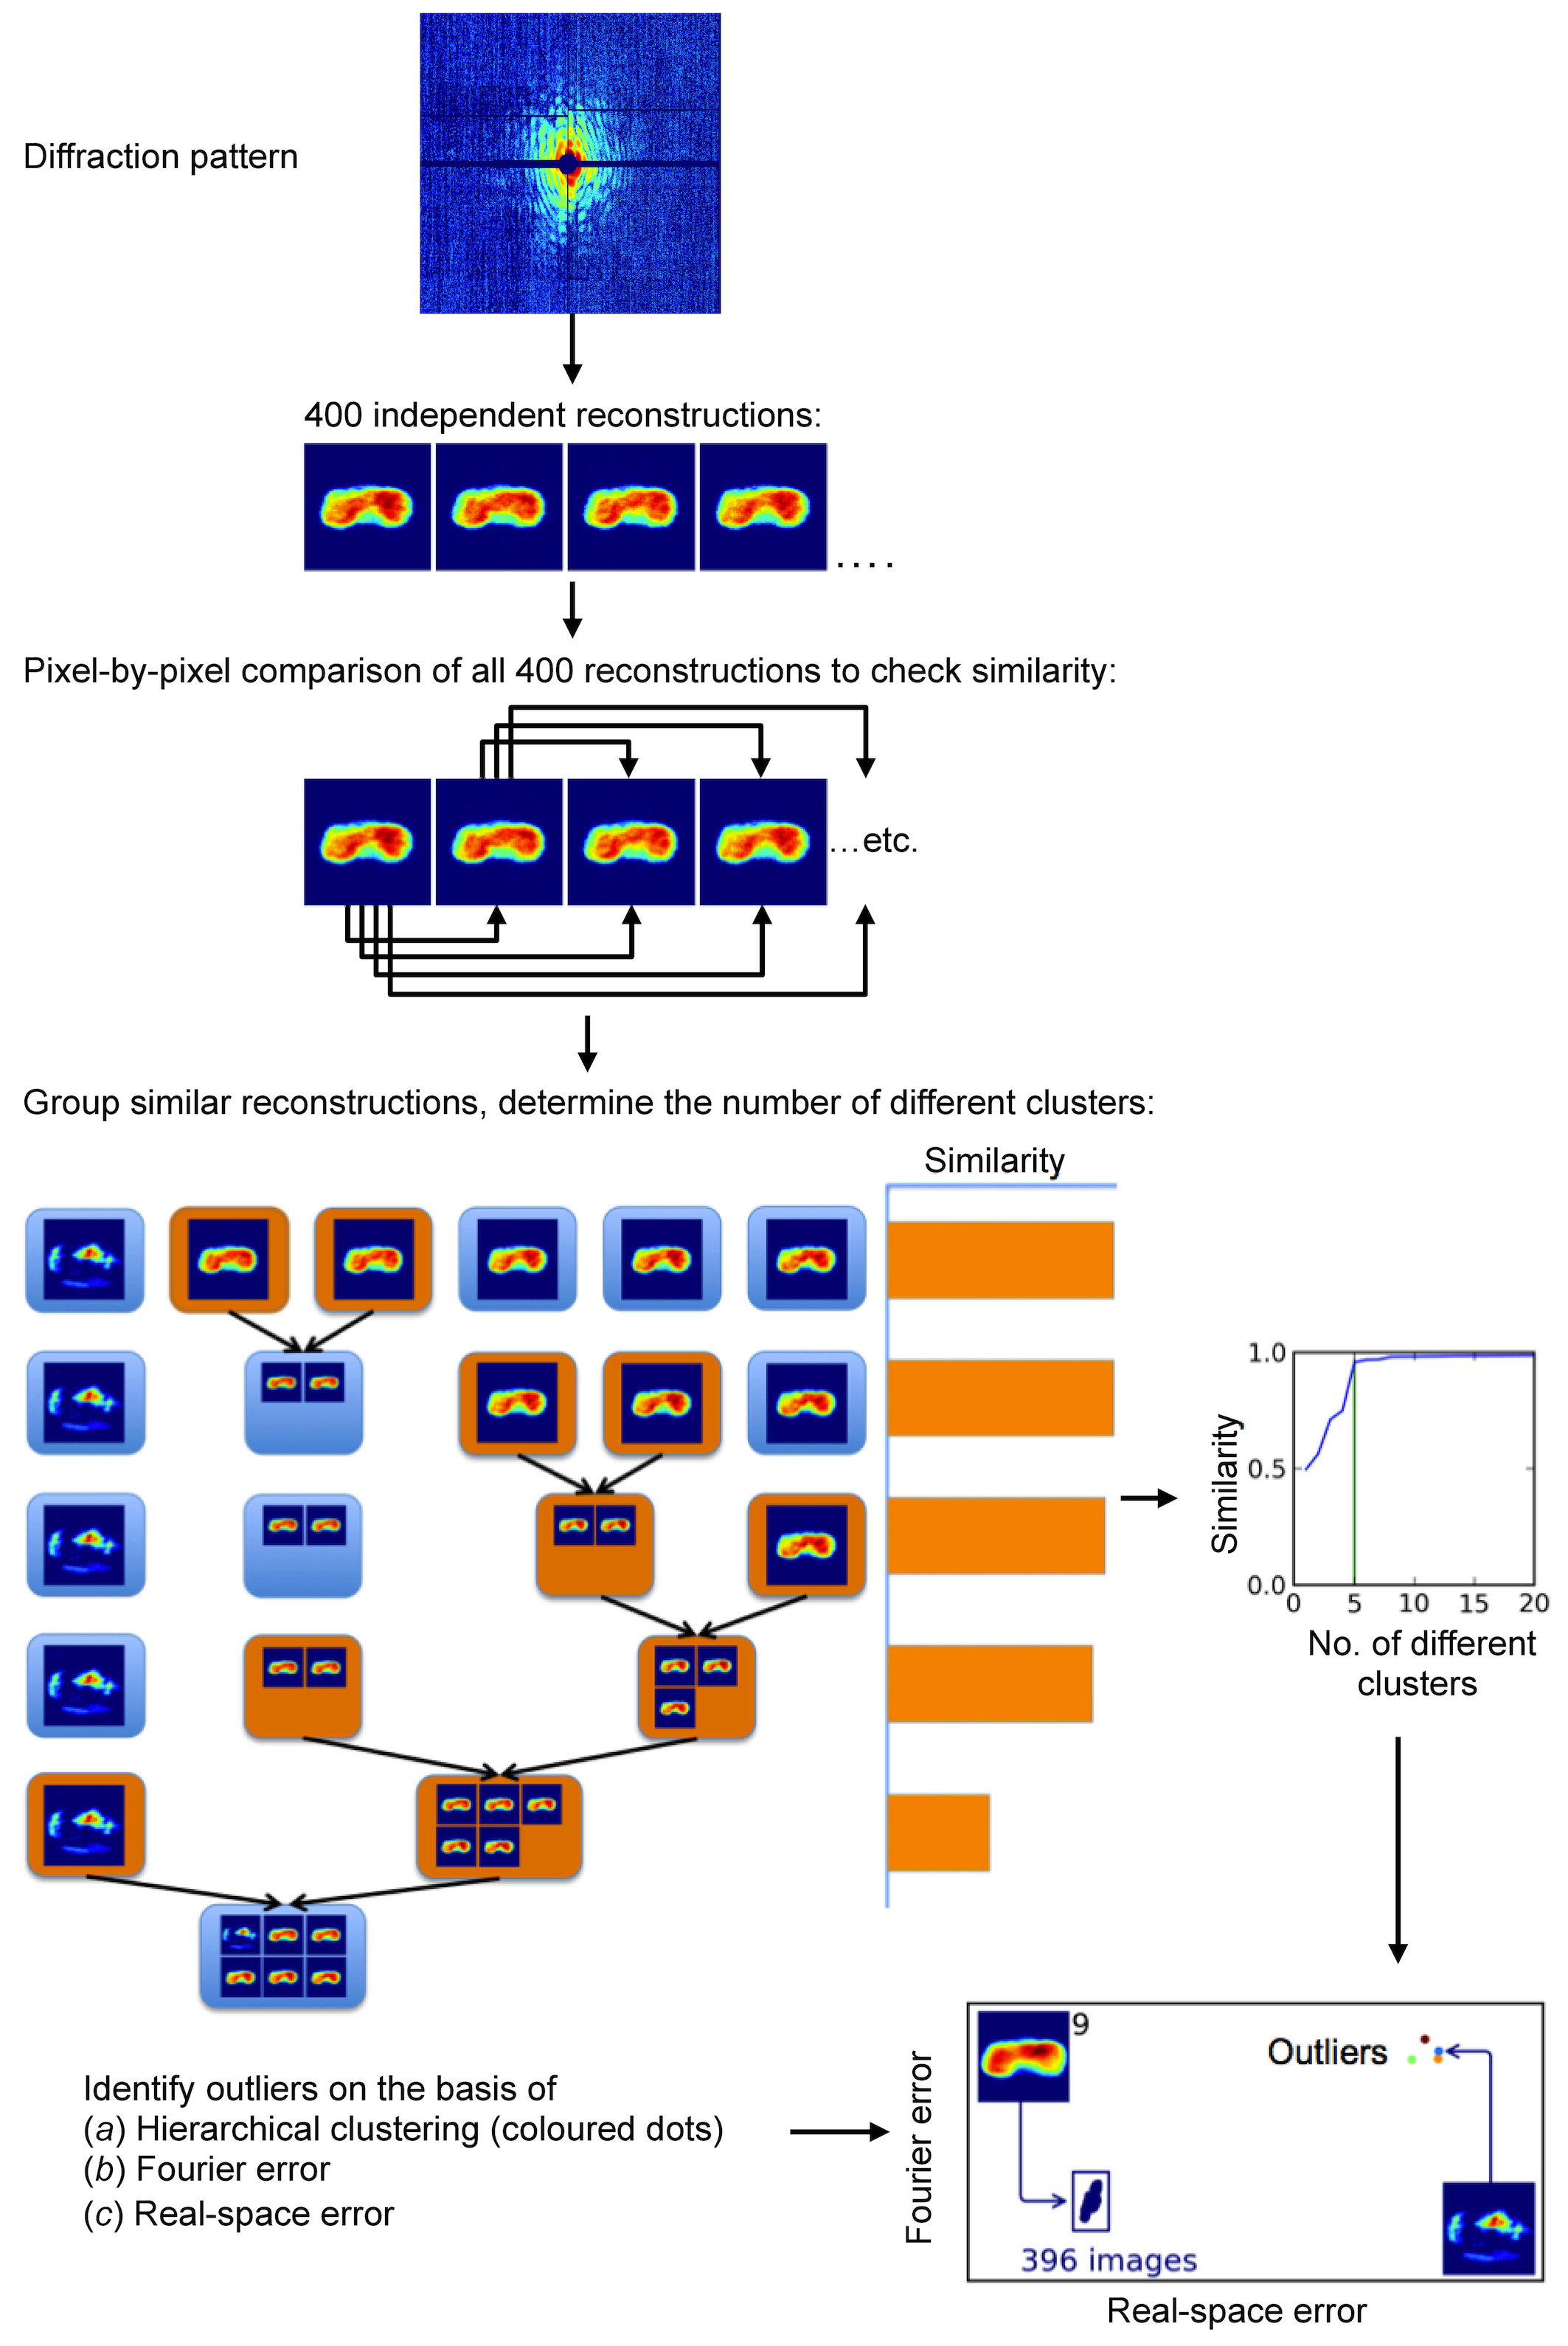
\includegraphics[width=100mm]{UPGMA_Clustering.jpg}
	\caption{UPGMA Clustering.}
	\label{fig:UPGMA}
\end{figure}

In the first step of this method each reconstruction is compared pairwise to every other reconstruction, pixel-to-pixel. The similarity score associated with each comparison is the normalized scalar product between the pair of reconstructions, after translating them to their optimal fit. 

In the second step of the method similar reconstructions are grouped in clusters. Initially each reconstruction belongs to its own cluster. In every consecutive step the two most similar clusters are merged into one cluster, until in the end only one big cluster remains. For each merge we calculate the average similarity score over all reconstruction in the merged cluster. We plot the average similarity score of each cluster merge as a function of the number of clusters. The agglomeration step where the plot makes a "kink" is chosen as the number of different clusters that are present in the set of reconstructions. This is a standard way to estimate the number of clusters present in the set of reconstructions. This capability is an advantage of the  clustering algorithm. 

In a 2D plot of $E_f$ vs. $E_r$, color-coded by cluster, it is possible to see whether or not there is a correlation of reconstruction similarity and error score.  In the case that several large clusters remaining after applying a real-space error and Fourier-error threshold the clusters have to be examined carefully. If the remaining clusters correlate with the errors we suggest to keep only the cluster with the lowest error. If no correlation is present between score and cluster it is advised to keep all clusters for further evaluation. Otherwise there is a possibility of selecting on similarity, which would negate the validation power of the PRTF.

 
\section{Simulated Phase Contrast Methods}
Once one has retrieved the phase of the diffraction pattern, one has complete knowledge of the information encoded in the said wave-field. This total knowledge is powerful, because it allows the emulation of the action of any imaging system for which an associated mathematical transform can be written, regardless of whether that system is experimentally realizable in hardware.

For example, differential interference contrast imaging or Nomarski imaging is experimentally a well established technique to visualize the changes in phase. This change can have biological meaning, as for example the density inside certain organelles can be higher than the average density in cells. Normarski imaging will give a more pronounced image of the borders of the organelle. For an example see ref [mitochondrium). 

Nomarkski imaging in its simplest form takes a coherent wave-field of interest, say $\psi(x,y,z = 0)$, and then interferes this wave-field with a copy of itself that has been given both a slight transverse displacement ($\Delta x$, $\Delta y$) and a phase shift $\phi_0$ (Nomarski and Weill,1955). Thus the intensity of the resulting wave-field is [Paganin]:
$|\psi(x,y,z=0)+ e^{(i\phi_0)} \psi(x - \Delta x,y - \Delta y,z=0) |^2$, from which one can show (using the Fourier shift theorem) that the transfer function becomes:
\begin{equation}
\begin{aligned}
\begin{split}
T_{DIC}(k_x, k_y, \tau) = 1 + e^{(i(\phi_0 - k_x \Delta x - k_y \Delta y))},\\
\tau = (\phi_0, \Delta x, \Delta y)
\end{split}
\end{aligned}
\end{equation}

In the case of a reconstructed image $\rho(\vec{r})$, the Normarski variant will look like:
\begin{equation}
N = \mathcal{F}^{-1} T_{DIC} \mathcal{F}(\rho(\vec{r}))
\end{equation}
We have created simulated Nomarski images of the reconstructed cell images shown in the results part.



